%% This is file `sample-sigconf.tex',
%% generated with the docstrip utility.
%%
%% The original source files were:
%%
%% samples.dtx  (with options: `sigconf')
% TODO: Change to review before submitting
\documentclass[sigconf]{acmart}
%% \BibTeX command to typeset BibTeX logo in the docs
\AtBeginDocument{%
  \providecommand\BibTeX{{%
    \normalfont B\kern-0.5em{\scshape i\kern-0.25em b}\kern-0.8em\TeX}}}

%% Rights management information.  This information is sent to you
%% when you complete the rights form.  These commands have SAMPLE
%% values in them; it is your responsibility as an author to replace
%% the commands and values with those provided to you when you
%% complete the rights form.
\setcopyright{acmcopyright}
\copyrightyear{2018}
\acmYear{2018}
\acmDOI{XXXXXXX.XXXXXXX}

%% These commands are for a PROCEEDINGS abstract or paper.
\acmConference[ICSE 2024]{46th International Conference on Software Engineering}{April 2024}{Lisbon, Portugal}
%
%  Uncomment \acmBooktitle if th title of the proceedings is different
%  from ``Proceedings of ...''!
%
%\acmBooktitle{Woodstock '18: ACM Symposium on Neural Gaze Detection,
%  June 03--05, 2018, Woodstock, NY} 
\acmPrice{15.00}
\acmISBN{978-1-4503-XXXX-X/18/06}

% My packages
\usepackage{orcidlink} % Orcid links

%%
%% end of the preamble, start of the body of the document source.
\begin{document}

%%
%% The "title" command has an optional parameter,
%% allowing the author to define a "short title" to be used in page headers.
\title{Implementing the Visual Debugger: An Experience report}

\author{Tim Kr\"{a}uter \orcidlink{0000-0003-1795-0611}}
\email{tkra@hvl.no}
\orcid{0000-0003-1795-0611}
\affiliation{%
  \institution{Western Norway University of Applied Sciences}
  \city{Bergen}
  \country{Norway}
}

\author{Adrian Rutle \orcidlink{0000-0002-4158-1644}}
\email{aru@hvl.no}
\orcid{0000-0002-4158-1644}
\affiliation{%
  \institution{Western Norway University of Applied Sciences}
  \city{Bergen}
  \country{Norway}
}

\author{Harald K\"{o}nig \orcidlink{0000-0001-6304-6311}}
\email{harald.koenig@fhdw.de}
\orcid{0000-0001-6304-6311}
\affiliation{%
  \institution{University of Applied Sciences, FHDW}
  \city{Hannover}
  \country{Germany}}
\affiliation{%
  \institution{Western Norway University of Applied Sciences}
  \city{Bergen}
  \country{Norway}
}

\author{Yngve Lamo \orcidlink{0000-0001-9196-1779}}
\email{yla@hvl.no}
\orcid{0000-0001-9196-1779}
\affiliation{%
  \institution{Western Norway University of Applied Sciences}
  \city{Bergen}
  \country{Norway}
}

% \author{Patrick Stünkel \orcidlink{0000-0002-0537-295X}}
% \email{patrick.stuenkel@hvl.no}
% \orcid{0000-0002-0537-295X}
% \affiliation{%
%   \institution{Western Norway University of Applied Sciences}
%   \city{Bergen}
%   \country{Norway}
% }

\renewcommand{\shortauthors}{Kräuter et al.}

%%
%% The abstract is a short summary of the work to be presented in the
%% article.
\begin{abstract}
  TODO: Abstract
\end{abstract}

\keywords{IDE, Plugin, IntelliJ IDEA Plugin, Experience Report, Debugging, Visual Debugging, Visual Debugger, Software Visualization}

\received{9 November 2023}
% \received[revised]{12 March 2009}
% \received[accepted]{5 June 2009}

\maketitle

\section{Introduction}

\begin{figure}[ht]
  \centering
  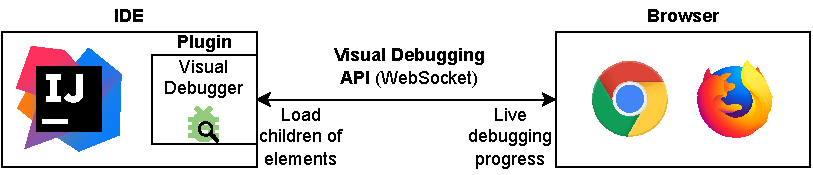
\includegraphics[width=\linewidth]{images/VD-architecture.pdf}
  \caption{Pic}
\end{figure}

\cite{krauterVisualDebuggerTool2022}

% \section{Acknowledgments}

\bibliographystyle{ACM-Reference-Format}
\bibliography{bib}
\end{document}
\endinput
%%
%% End of file `sample-sigconf.tex'.
